\documentclass[14pt, a4paper]{article}


\usepackage{geometry}
 \geometry{
 a4paper,
 total={170mm,257mm},
 left=20mm,
 top=10mm,
 }
\usepackage{graphicx}


	\begin{document}
		
				
		\title{\textbf{ WI-FI DISTRIBUTIONS AND THEIR INFORMATION STATUS}\\A SURVEY BASED ON WIFI-HOTSPOTS AROUND MAKERERE UNIVERSITY }

		
		\author{LUKWAGO HASSAN NASSIL  216005795 16/U/6666/EVE}

		\date {\today}

		\maketitle

			\section{Acknowledgements}
I wish to thank Makerere University for allowing me access and to document their WI-FI hotspot information.  In particular, I wish to thank Professor Engineer Bainomugisha.  the Head of Department Computer Science, for his keen interest and guidance in the development of this study.\\



I would like to thank the all the students  for their contribution to the gathering of information about WI-FI hotspot information and preparation of this report.\\



I also wish to thank my supervisor, Professor Earnest Mwebaze for the academic support and assistance throughout the writing of the report.\\



Finally, I wish to thank my family and friends for their unending love and encouragement throughout this process.  I am and will remain eternally grateful.\\


		\tableofcontents


			\section{Tables}
Table 1 Methods used to answer research questions	............................. 4\\


			\section{Figures}
Figure 1 Chart title	......................................................................4\\



			\section{Acronyms}
WI-FI 		Wireless Fidelity\\
SSID 		Social Security Identification\\
XML		Extensible Mark-up Language \\
ODK		Open Data Kit\\			


			\section {Executive Summary}
				\subsection{Background}
There have been reported cases concerning freshmen students of Makerere  university not knowing which WI-FI (Wireless Fidelity) networks they are entitled to use, this has been a main concern as according to the tuition structure, there is a noticeable percentage of the tuition that is allocated for internet usage (both wired and wireless). Thus every student of the great Makerere is entitled to the information and data that was collected during this research. This data will be uploaded on a cloud server where developers, network administrators can be able to access it and thus will lay ground to their project implementations. 

				\subsection{Methodology}

The data in this research was collected using electronic methods. An XML (Extensible Mark-up Language ) was created and uploaded on an aggregate server, the link to the aggregate entered in an android application(ODK collect) to link up the smart phone application to the server. The application retrieved a copy of the form and created bank multiple bank forms that where used as questionnaires for entering the WI-FI information

				\subsection{Key Findings}
In seeking to understand the Wi-Fi passwords, it was found out that most of the hotspots in Makerere university are not for students use but rather their passwords are concealed for private use and a big number of such hotspots where found out in the Makerere grounds. On obtaining the data for the research project, the following where noticed.\\

•	Some students did not know the password of the that they are connected to as the tend to forget them since they only require them during the first time they are connecting to the Wi-Fi, thus taking time to find a student who knows the password.\\

•	A number of Wi-Fi hotspots are in door located and thus giving a hard time to track and record the GPS readings of the device in the location.\\

				\subsection{Key Recommendations}


•	After centrally managing the database on a server, there is still a problem of freshmen accessing the link to the centrally managed database and a better way of solving this problem is by making Wi-Fi hotspots open.\\


•	Basing on the result, setting up an online server itself is not enough and to solve this problem can be solved by hiring developers to create web and mobile applications that will make efficient use of this data and easily accessible to all the university students.\\


•	Another proper way of publishing Wi-Fi hotspots is to pinpoint the coordinates generated for the different Wi-Fi hotspots on google map along with some common characteristics of within the university to provide a good identification. \\

				\section{Introduction}

This research has been conducted mainly to save students the burden of searching for Wi-Fi hotspots location and passwords for the protected hotspots. This research will solve this problem by creating a database that will be managed centrally on an online site (http://project-167910.appspot.com )hosted by googleAppEngine and this information gathered will be open source that can be accessed by Makerere university students, Network Administrators, Application developers and other people that would like to acquire it.\\

				\subsection{Objectives}

The objectives of Wi-Fi distributions and their information status around Makerere university research project are to:\\


1)	To obtain a database about the different Wi-Fi hotspots around Makerere university that will be centrally managed by the Network Administrators of the University.\\


2)	To provide all the student of Makerere university with all the Wi-Fi SSID names along with their passwords for those that are accessible by the students.\\

3)	To save time by laying ground for the mobile and application developers that may need this information as a subsidiary in their projects.\\

4)	To accurately locate and provide the geo position of the hotspots that are located within Makerere university ground.\\

5)	To give students a chance to maximize and utilize the resources of the university that they are entitled to.\\

				\section{Methodology}

				\subsection{Research Questions}

The research questions to be answered are:\\

1.	What is the WI-FI name(SSID)?\\

2.	What is the WI-FI password?\\

3.	What is the current geo position.\\

4.	Take a photo of location.\\

5.	Enter the coverage radius in meters.\\

6.	What is the WI-FI type?\\

7.	How many bars do you record currently?\\

8.	Is the Wi-Fi indoor or outdoor?\\

9.	What are the maximum number of users?\\



				\subsection{Research Design}

The interviewee will use qualitative, quantitative, mixed methods to answer the research questions. The following table summarises the methods used to answer each question:\\

\begin{tabular}{||c|c||}
\hline Research Question &  Method Used to Answer Question\\
\hline What is the WI-FI name(SSID)? & Qualitative\\
\hline What is the WI-fFI password? & Qualitative\\
\hline What is the current geo position & Quantitative\\
\hline Take a photo of location & Qualitative\\
\hline Enter the coverage radius in meters. & Quantitative\\
\hline How many bars do you record currently? & Quantitative\\
\hline Is the WI-fi indoor or outdoor? & Qualitative\\
\hline What are the maximum number of users? & Quantitative\\
\hline
\end{tabular}

			\subsection{Instruments}

\textbf{Aggregate server}: this was used a platform to centrally manage the data, and every data that was collected was sent to this server and can later be used for visualization.\\

\textbf{ODK collect}: A mobile application that was used to enter the data collected including geo position of each entry and a pic of the pace from which data was obtained.\\

\textbf{XML FORM BUILDER}: this is an online plat form that created the form named wifi form and giving data values to each entry.\\


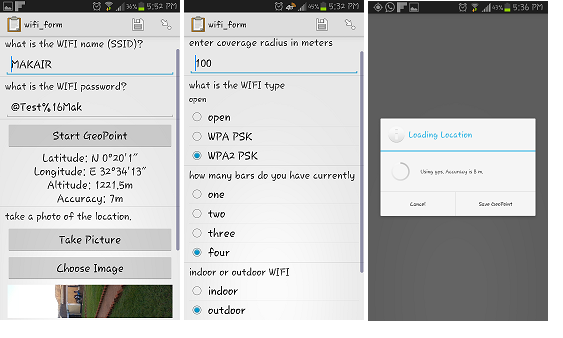
\includegraphics{d}

			\subsection{Sample}


The hotspots information was obtained by sampling every location around the Makerere grounds and a WI-FI tester was used to view every hotspot that has no hidden attribute to come up with the information.\\

			\subsection{Data Collection}

The data was collected both face-to-face and by phone where the sudents found accessing any wifi would be interviewed to obtain both the SSID and the confidential information and the rest of the data inputs where obtained as follows.\\

i)	Geo position was obtained using the satellite readings on the application while running on the smart phone.\\
ii)	The coverage radius was obtained by measuring the distance from the Wi-Fi router up to when the Wi-Fi signal reading is lost on the android smart phone.\\

iii)	The Wi-Fi type was recorded from the device connected the it and this had any of the three types open, WPA PSK and WPA2 PSK.\\

iv)	The bar signal which denotes the signal strength was also obtained the smart phone reading.\\

v)	The photo of the location was obtained by using the camera of the phone.\\

vi)	The maximum number of users was obtained by getting the number of users the Wi-Fi router could accommodate.\\


			\subsection{Data Analysis}

After collecting the data using the ODK collection tool, an internet connection would later be used to upload the obtained entries directly on the aggregate server which is on the site http://project-167910.appspot.com. On the same site, the data visualization of bar graphs, pie charts and map view of the coordinates \\

			\subsection{Limitations}

This research does not include all hotspot security keys that are not for the student, some hotspot are for the teaching and others are for payment(business) and thus only the SSID is provided and the key is set to confidential.\\
This research project does not include Wi-Fi hotspots that are outside Makerere University grounds.\\


			\section{Results}

			\subsection{The ratio of indoor to outdoor Wi-Fi hotspots}
It was found out that 62.3 percent of the Wi-Fi hotspots are located outside of the Makerere university and this is due to a duplicated number of MAKAIR hotspot that was found out in most of the campus grounds\\

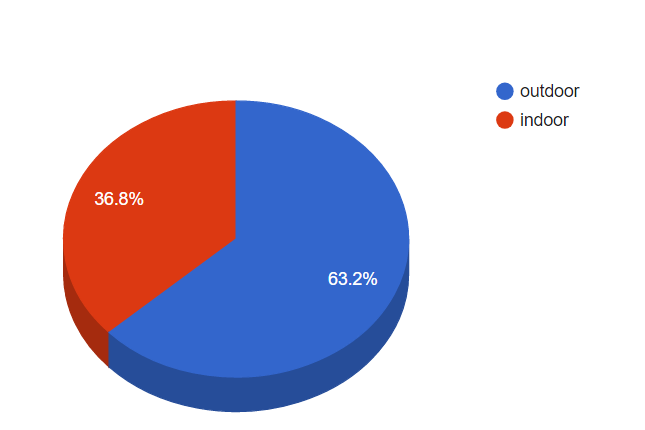
\includegraphics{io}

			\subsection{What is the most dominating Wi-Fi type?}
According to the collected data, it was found out that the ratio of WPA2 PSK Wi-Fi is the highest and the author interviewed the network administrator about this, he was replied that this was intentionally made to prevent hackers, and outside student from maliciously accessing the Wi-Fi hotspots as they could tap directly into the students registration and graduation system and hack the data.

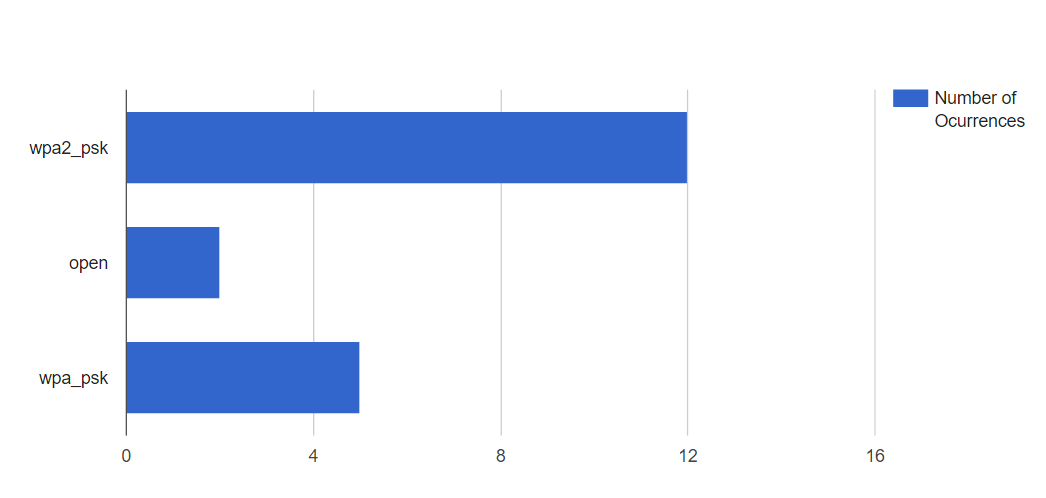
\includegraphics{wt}


			\section{Discussions}
According to the results in the previous section, it is found out that the protected Wi-Fi (both WPA PSK and WPA) are dominating the open Wi-Fi hotspots and this is sufficient information to show that there is no way a freshman can acquire confidential acces of the different hotspots located with in makerere university.\\

			\section{recommedations}
Based on the results from the research project about the Wi-Fi distribution and their information status the following recommendations are made:\\

•	After centrally managing the database on a server, there is still a problem of freshmen accessing the link to the centrally managed database and a better way of solving this problem is by making Wi-Fi hotspots open.\\

•	Basing on the result, setting up an online server it self is not enough and to solve this problem can be solved by hiring developers to create web and mobile applications that will make efficient use of this data and easily accessible to all the university students.\\

•	Another proper way of publishing Wi-Fi hotspots is to pinpoint the coordiates generated for the diffent wi-Fi hotspots on google map along with some common charactrictics of with in the university to provide a good identification. \\

		\section{References}
$[1]https://dicts.mak.ac.ug/services/wireless-accessi$\\
$[2] http://wifi-project-167910.appspot.com $\\


			

				
	

	\end{document}
